\documentclass[../main.tex]{subfiles}
%!TEX root = ./appendixGUI.tex
\graphicspath {{../}}

\begin{document}
\chapter{Instructions for Installing and Running the GUI} \label{appendix:GUI}

Running the GUI involves simply running the main.m file. Ensure that the current folder on MATLAB is the one containing the main.m file. Simply adding it to the path will cause errors when trying to write to the text files. Upon running main.m the GUI will launch as shown in Figure \ref{fig:gui}. In terms of inputs, there are default selected values and the program can be run by pressing the Generate button.

\begin{figure}[H]
	\centering
	\includegraphics[width=\linewidth]{img/gui/gui.pdf}
	\caption{Overview of te Entire GUI}
	\label{fig:gui}
\end{figure}

The GUI is broken into different sections based on their use. These are labels in Figure \ref{fig:gui} correspond to the list below. The description of each of the areas is:

\begin{enumerate}
	\item Envelope Dimensions: fields to enter dimensions of the envelope, discussed in Section \ref{gui:envelope}.
	\item Main Parameters: the three main inputs for the program, discussed in Section \ref{gui:parameters}.
	\item Important Value: an output of the important parameters of the program. These are also found in the log but are displayed here, so they can easily be seen after the program is run.
	\item Log: the log section takes the text from the log file and displays it here once the program is completed.
	\item Graphs: the right side of the GUI will display useful graphs of the airship that was generated. The top one with the drag and thrust curve. The difference between the two is the acceleration of the airship and their intersection is the maximum possible speed.
\end{enumerate}

\section{Entering Envelope Dimensions} \label{gui:envelope}
As mentioned above this section allows the user to input the dimensions of the envelope. A close up of the section can be seen in Figure \ref{fig:gui1}.

\begin{figure}[H]
	\centering
	\includegraphics[width=0.7\linewidth]{img/gui/guiSection1.pdf}
	\caption{Close Up of the Envelope Dimensions}
	\label{fig:gui1}
\end{figure}
\begin{enumerate}[	A]
	\item Length: the tip to tip length of the airship in metres.
	\item Diameter: the diameter of the main cylinder of the airship in metres.
	\item Fineness Ratio: the ratio between the the length and the diameter of the airship.
	\item Section Length: calculated value of the length of the cylindrical shape of the blimp. Used to make sure it is within the limits of 1m to 1.524m.
	\item Calculate: button that runs the calculation of the dimensions, it will NOT run the full program.
\end{enumerate}

Since the three input fields are all related, only two fields need to be filed out to calculate the airship dimensions. In the case where all three are input, the default will be to use the Length and Fineness Ratio. The errors from this section will appear as a message box or in the Main Parameters Section \ref{gui:parameters}, they are all outline in Section \ref{gui:error}

\section{Entering Main Parameters} \label{gui:parameters}
This section of the GUI is the inputs for the main parameters of the program. These are the required weight, required speed, and flight time. This can all be seen in Figure \ref{fig:gui2} below.

\begin{figure}[H]
	\centering
	\includegraphics[width=0.7\linewidth]{img/gui/guiSection2.pdf}
	\caption{Close Up of the Main Parameters}
	\label{fig:gui2}
\end{figure}

\begin{enumerate} [	A]
	\item Dominant Parameter: selects the parameter the program will attempt to achieve.
	\item Required Weight: the required carrying capacity of the airship.
	\item Required Speed: the required top speed of the airship.
	\item Required Flight Time: the required flight time of the airship
	\item Generate: this button will run the program. It will also run the calculations of the envelope size, so the calculate button doesn't necessarily have to be pressed before the generate button.
	\item Values: this section shows the values of the sliders.
	\item Warning: this will show warnings about the envelope dimensions. They are listed in section \ref{gui:error}.
\end{enumerate}

\section{Warnings and Errors} \label{gui:error}
To try to prevent errors occurring in the code and in the SolidWorks, warnings and errors are added to the code. These use message boxes and text on the GUI to display this information. The first type of warning are the ones displayed on the GUI these can be seen in Figure \ref{fig:warningDimensions}. None of these warning will prevent the user from running the program.

\begin{figure}[H]
	\centering
	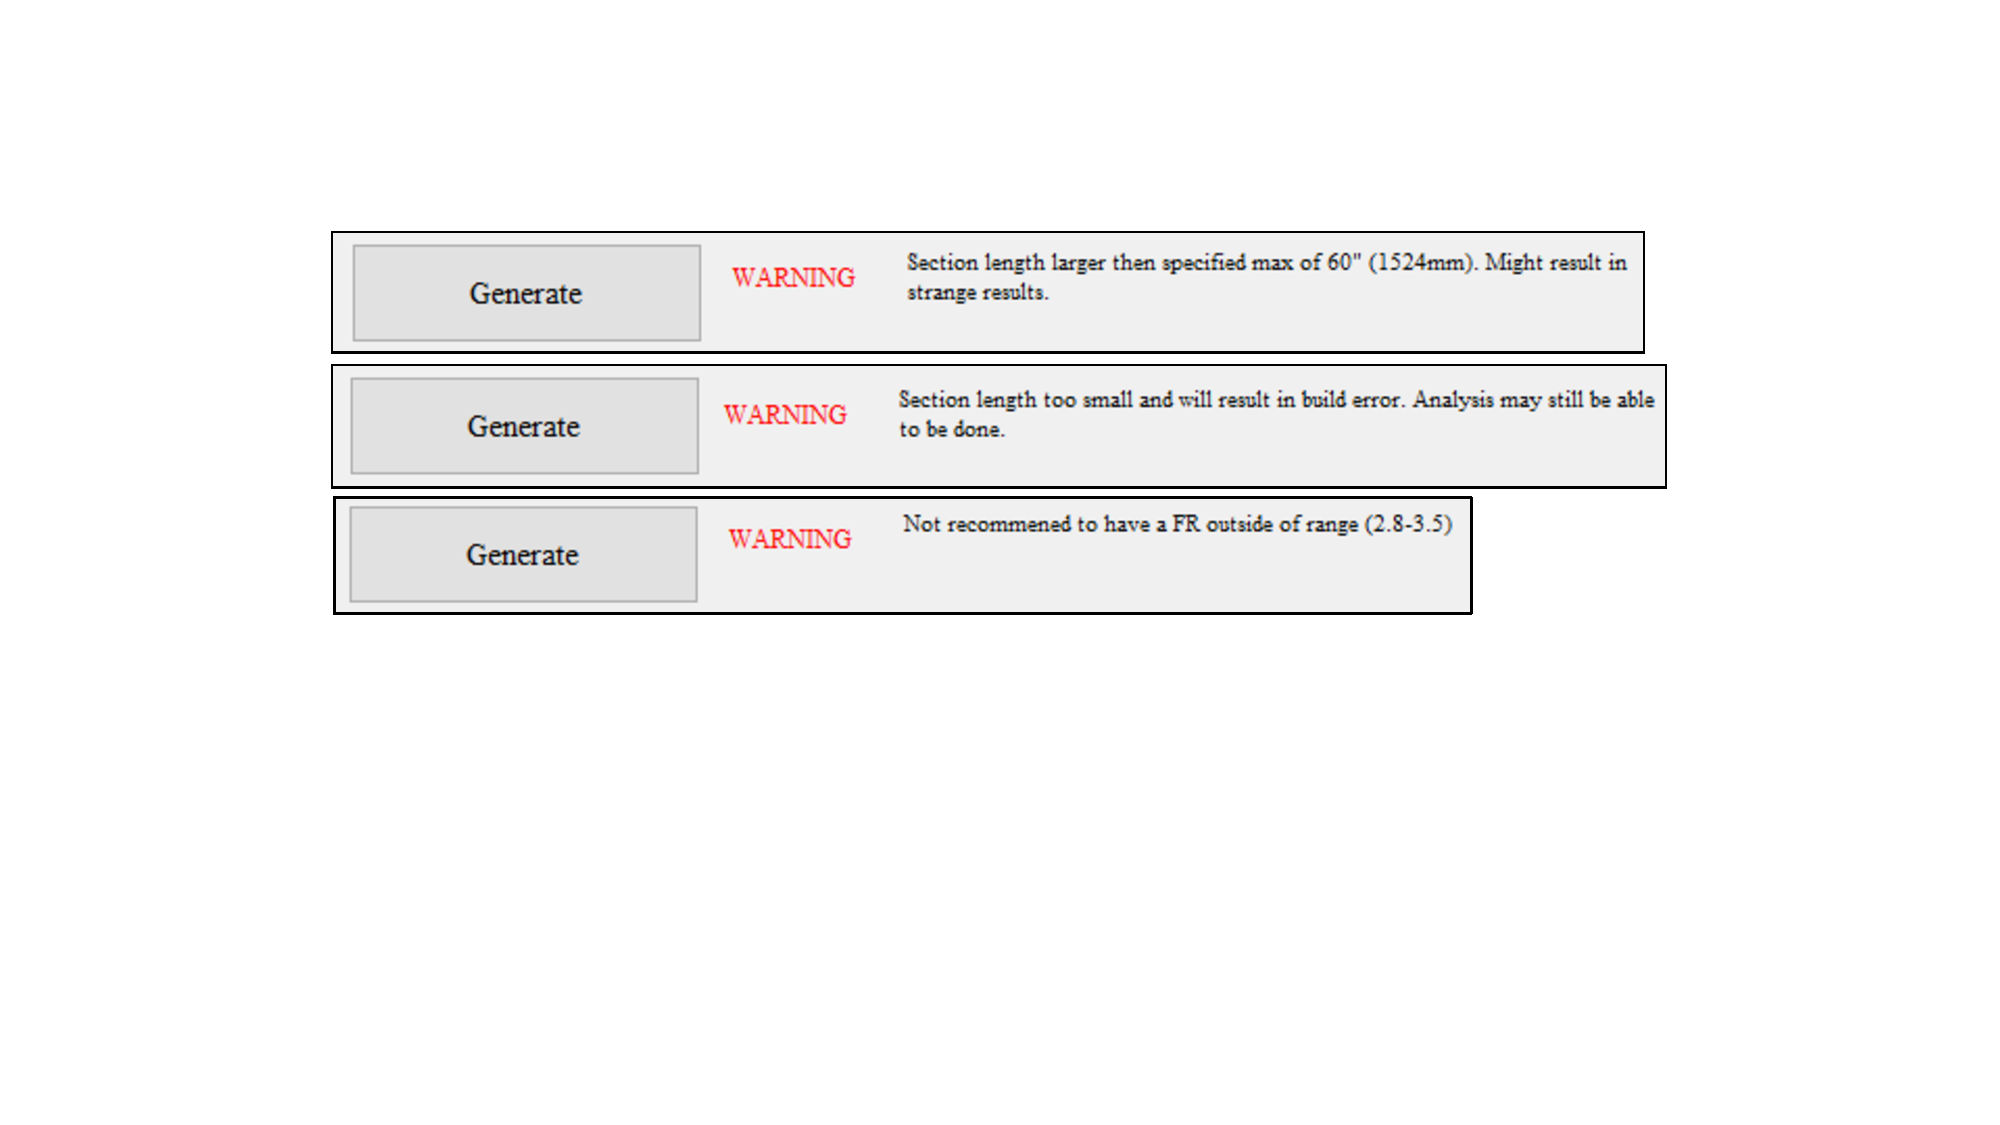
\includegraphics[width=0.9\linewidth]{img/gui/dimensionWarnings.pdf}
	\caption{Dimension Warnings on the GUI}
	\label{fig:warningDimensions}
\end{figure}

\begin{enumerate}
	\item \textbf{Large Section Length} is caused by the section length of the blimp being larger than the specified maximum length. The code should still optimize the dimensions, however it wasn't particularly tested past this value and some unexpected results may occur.
	\begin{itemize}
		\item Fix: Reduce the Length and/or the Fineness Ratio.
	\end{itemize}
	\item \textbf{Small Section Length} is caused by the section length of the blimp being less than $1m$ this will cause issues with the SolidWorks since the thruster will try to be places on the cone section and fail. In general the airship is fairly small and will likely be unable to carry the components.
	\begin{itemize}
		\item Fix: Increase the Length and/or the Fineness Ratio.
	\end{itemize} 
	\item \textbf{Fineness Ratio} this is caused by a fineness ratio being outside the set range. The range was set for general look of the airship as well as the drag data being based on data points in this range. As long as the code is run close to to this range, there shouldn't be any problems.
	\begin{itemize}
		\item Fix: Change the Length and/or Diameter. Alternatively set the fineness ratio to a value in the range.
	\end{itemize} 
\end{enumerate}

The other types of warnings are from a message box, which pops up at the end of the program. They are there to warn the user if the program could not meet the specifications based on the inputs. The possible ones can be seen in Figure \ref{fig:popupWarnings}.

\begin{figure}[H]
	\centering
	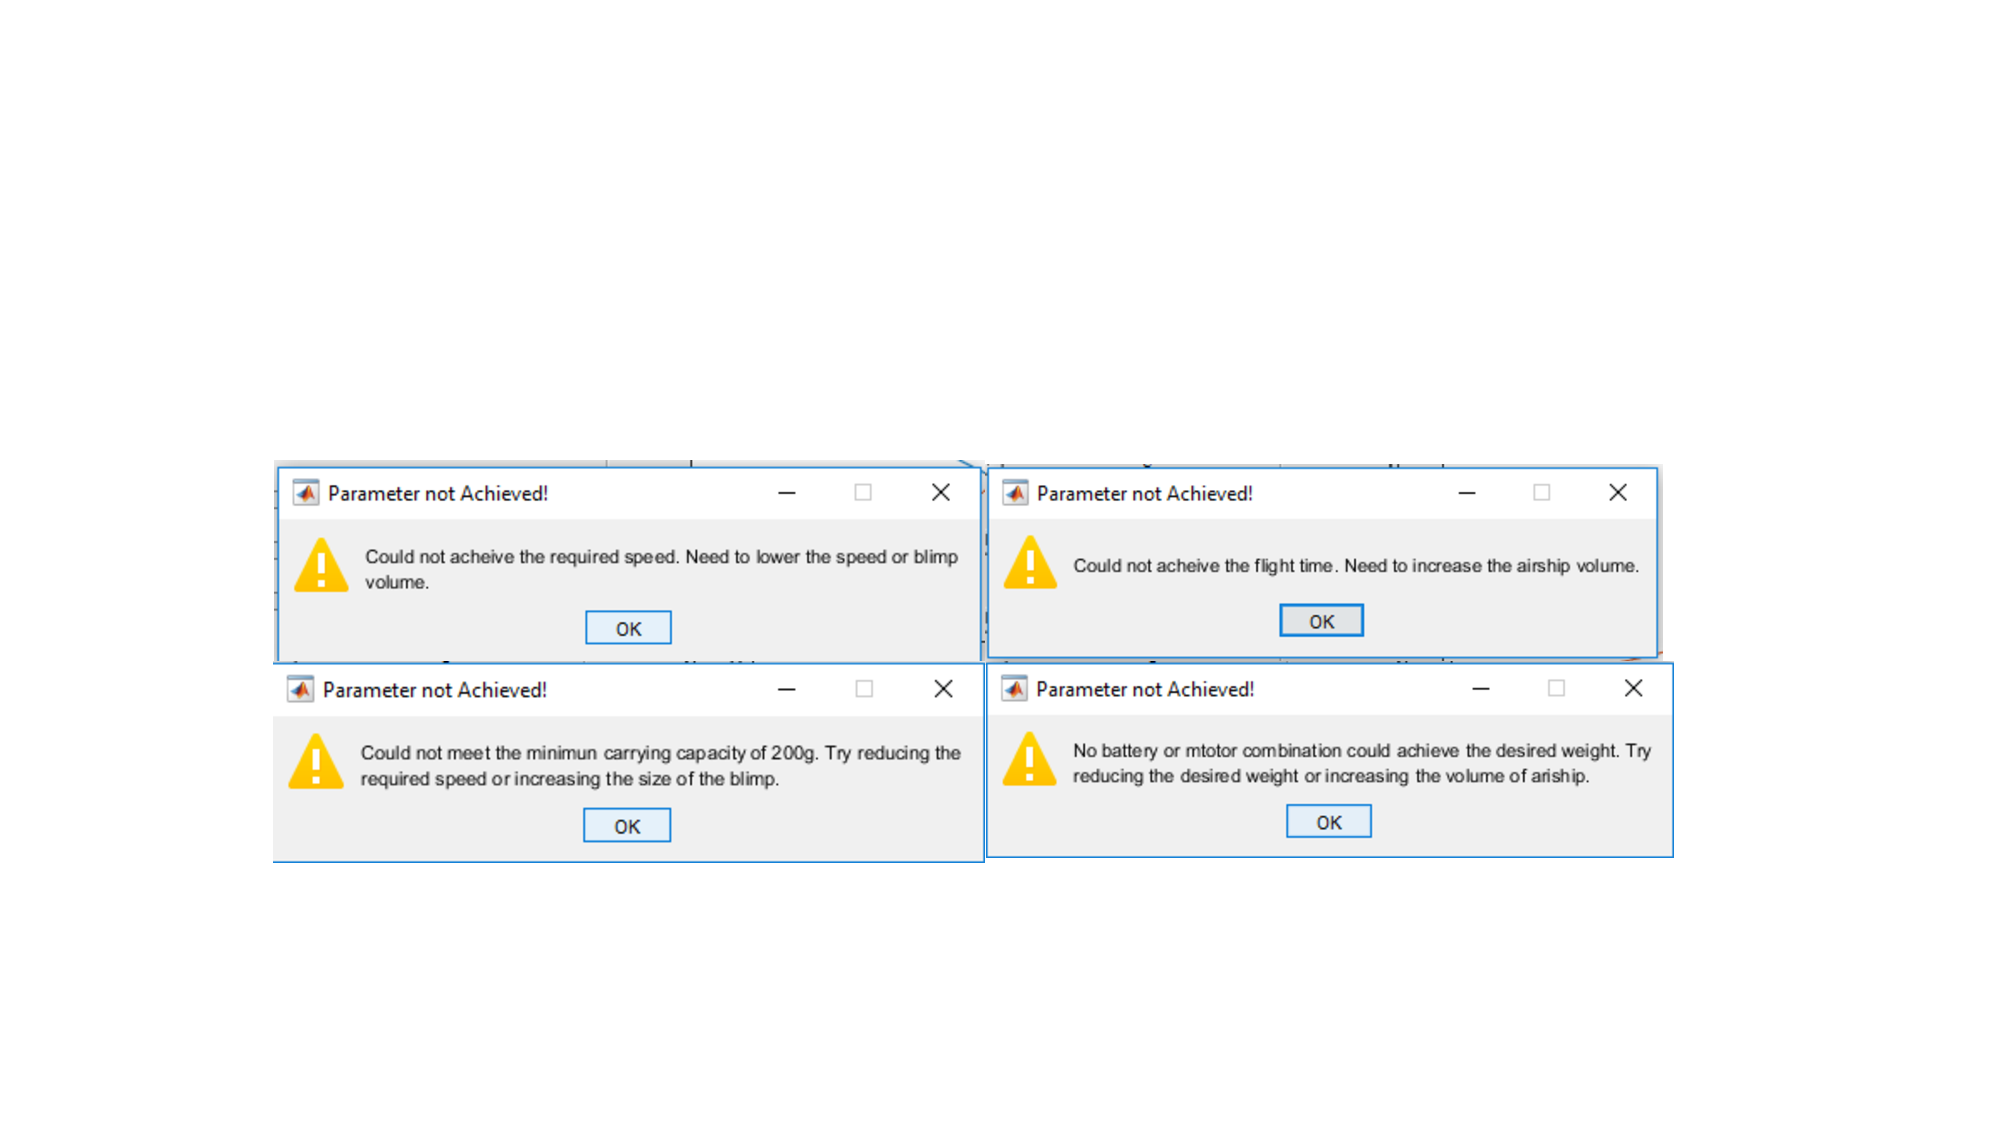
\includegraphics[width=0.9\linewidth]{img/gui/warnings.pdf}
	\caption{End Warnings Pop-Ups on the GUI}
	\label{fig:popupWarnings}
\end{figure}

\begin{enumerate}
	\item \textbf{Required Speed} occurs if the required speed is not met. This is unlikely to occur since the slider is roughly set to the maximum speed it can achieve
	\begin{itemize}
		\item Fix: Reduce the speed or reduce the size of the airship to lower the drag.
	\end{itemize}
	\item \textbf{Flight Time} occurs if the flight time is not met. This is also unlikely to occur since the slider is capped at the largest battery.
	\begin{itemize}
		\item Fix: Reduce the flight time
	\end{itemize} 
	\item \textbf{Minimum Carrying Capacity} occurs when the parameters input result in the blimp having a carrying capacity lower than the required.
	\begin{itemize}
		\item Fix: Increase the volume of the airship.
	\end{itemize} 
	\item \textbf{Required Weight} occurs when the carrying capacity could not be met.
	\begin{itemize}
		\item Fix: Increase the volume of the airship.
	\end{itemize} 
\end{enumerate}

The last set of warnings are the errors, which is major issues with the input parameters. These will need to be fixed and if they occur before the program is run, it will not allow it to run. The possible ones are shown in Figure \ref{fig:errors}.

\begin{figure}[H]
	\centering
	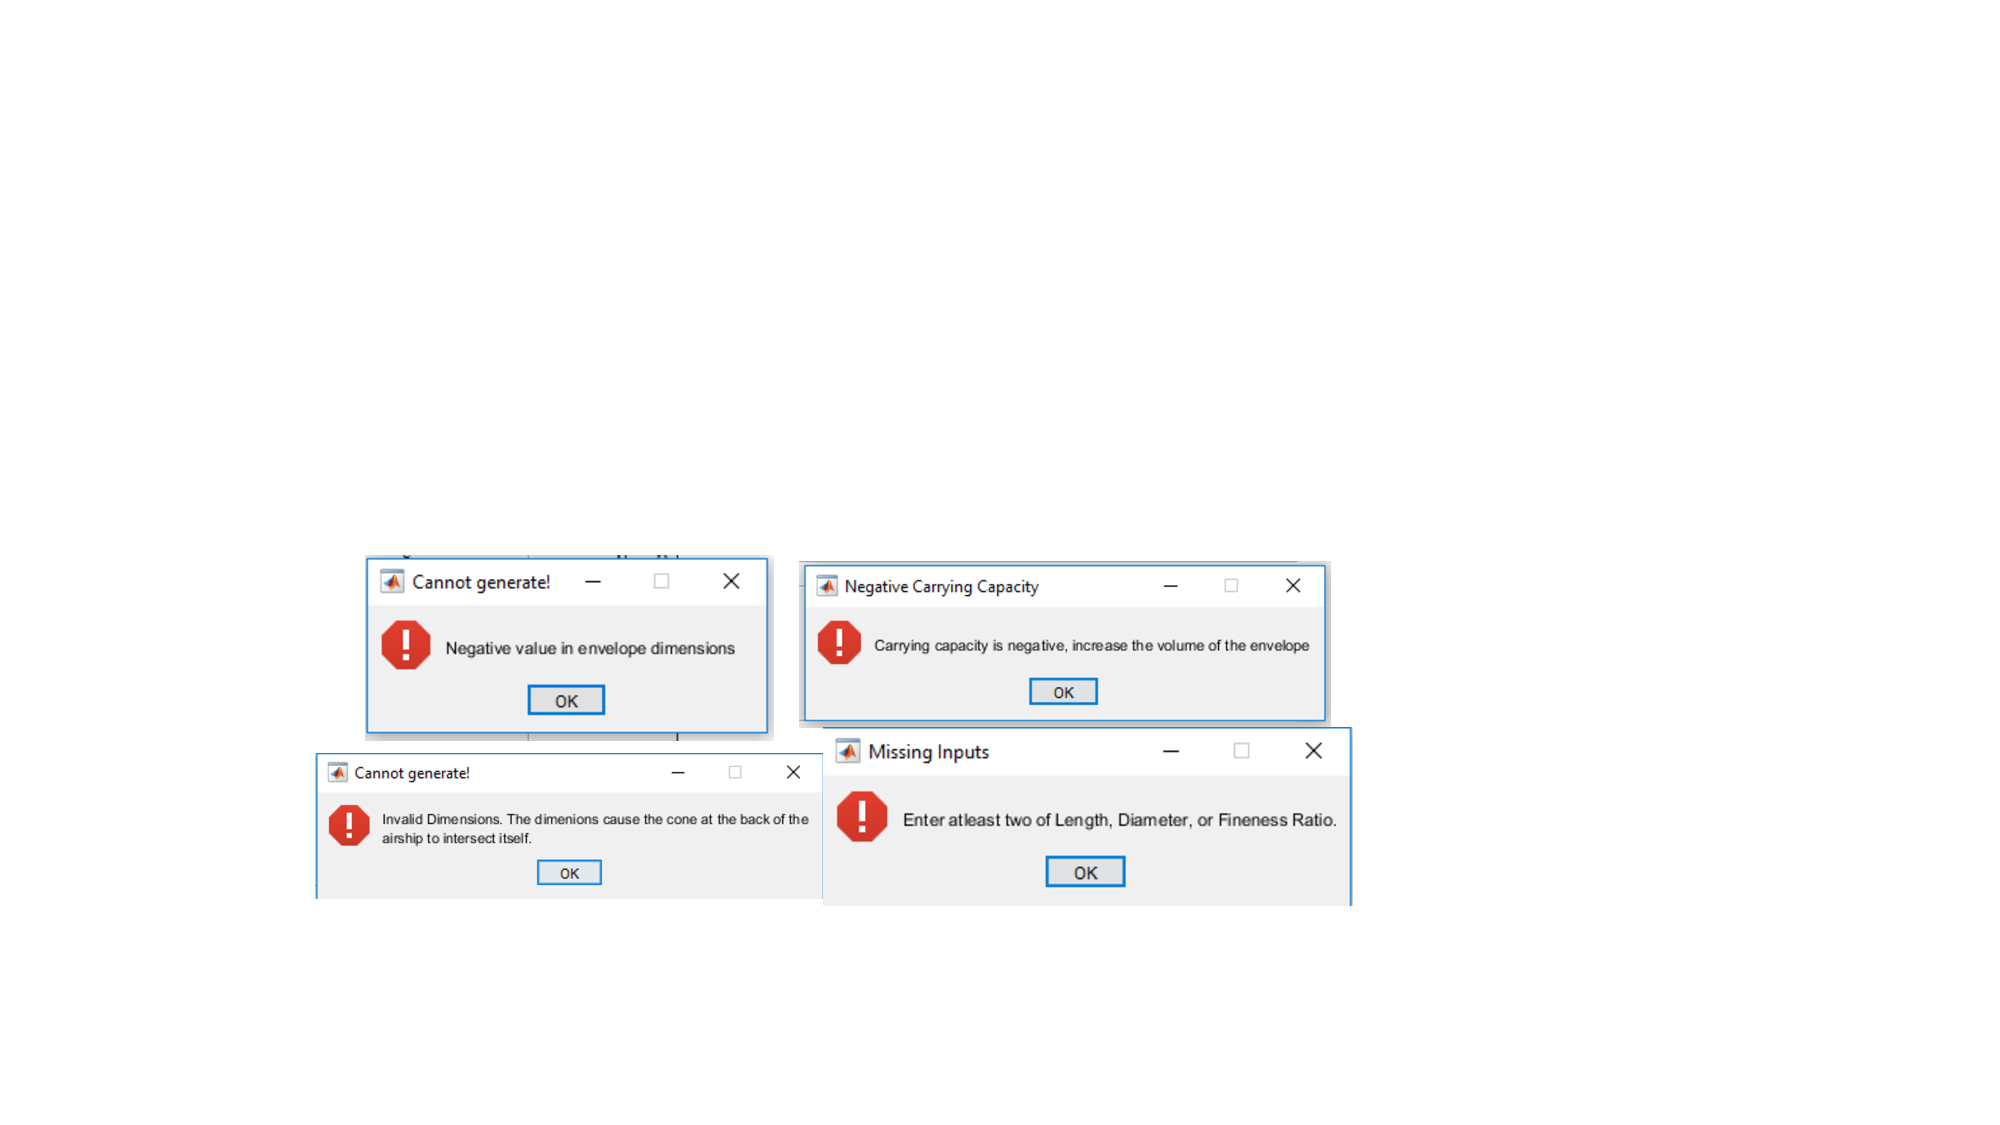
\includegraphics[width=0.8\linewidth]{img/gui/errors.pdf}
	\caption{End Warnings Pop-Ups on the GUI}
	\label{fig:errors}
\end{figure}
\begin{enumerate}
	\item \textbf{Invalid Dimensions} occurs if the dimensions cause the cone at the back to intersect itself.
	\begin{itemize}
		\item Fix: Reduce the fineness ratio of the airship.
	\end{itemize}
	\item \textbf{Carrying Capacity} occurs if the net weight of the airship is negative.
	\begin{itemize}
		\item Fix: Increase the volume of the airship.
	\end{itemize} 
	\item \textbf{Enter Two Dimensions} occurs when there is less than two of the input parameters.
	\begin{itemize}
		\item Fix: Enter two of the three dimensions
	\end{itemize} 
	\item \textbf{Negative Dimension} occurs when a negative value is input.
	\begin{itemize}
		\item Fix: Only input positive values
	\end{itemize} 
\end{enumerate}

\pagebreak
\end{document}